\documentclass[a4paper,titlepage,12pt]{article}
\usepackage[utf8]{inputenc} %Make sure all UTF8 characters work in the document
\usepackage{color}
\usepackage{graphicx}
\usepackage{titling}
\usepackage{tabularx}
\usepackage{longtable}
\usepackage[yyyymmdd]{datetime}
\usepackage[figurename=Figur]{caption}
\usepackage{pbox}
\usepackage{booktabs}

%Set page size
\usepackage{geometry}
\geometry{margin=3cm}

\renewcommand{\dateseparator}{-}
\renewcommand{\contentsname}{Innehållsförteckning}

%%%%%%%%%%%%%%%%%%%%%%%%%%%%%%%
% Header and footer
%%%%%%%%%%%%%%%%%%%%%%%%%%%%%%%
\usepackage{fancyhdr}
\pagestyle{fancy}

\lhead{
\includegraphics[width=0.15\linewidth]{images/logo_full.png}}
\chead{Systemskiss för sexbent robot}
\rhead{\today}
\setlength\headheight{26pt} 

\lfoot{TSEA29 --- KMM \\ LIPS Systemskiss}
\rfoot{Grupp 9 \\ LiTHe Hex}

\pretitle{%
    \begin{center}
        \LARGE
        
\includegraphics[width=6cm]{images/logo_full.png}\\[\bigskipamount]
}

\posttitle{\end{center}}

\begin{document}
    \title{\LARGE
        \textbf{Systemskiss för sexbent robot} \\
        \vspace*{0.5\baselineskip}
        \large
        Redaktör Frans Skarman \\
        Grupp 9 \\
        \small
        \vspace*{0.5\baselineskip}
        Version 0.1}

    \date{\today}

	\maketitle
	
	\newpage
	
	\begin{center}

		%%%%%%%%%%%%%%%%%%%%%%%%%%%%%%%%%%%%%%%%%%%%%%%%%%%%%%%%%%%%%%%%%%%%%%%%%%%%%%%%%
		%						Medlemmar
		%%%%%%%%%%%%%%%%%%%%%%%%%%%%%%%%%%%%%%%%%%%%%%%%%%%%%%%%%%%%%%%%%%%%%%%%%%%%%%%%%

		\section*{Projektidentitet}
		Grupp 9, Ht 2016, LiTHe Hex

		Linköpings Tekniska Högskola, ISY

		\begin{table}[h]
			\begin{center}
				\begin{tabular}[pos]{ l l l }
					\textbf{Namn} & \textbf{Ansvar} & \textbf{E-post} \\ \midrule
					Emil Segerbäck & & emise935@student.liu.se \\ \midrule
					Frans Skarman & Dokumentansvarig & frask812@student.liu.se \\ \midrule
					Hannes Tuhkala & & hantu447@student.liu.se \\ \midrule
					Malcolm Vigren & Projektledare & malvi108@student.liu.se \\ \midrule
					Noak Ringman &  & noari093@student.liu.se \\ \midrule
					Olav Övrebö &  & olaov121@student.liu.se \\ \midrule
					Robin Sliwa &  & robsl733@student.liu.se \\
				\end{tabular}
			\end{center}
		\end{table}

		\centering
		\textbf{Kursansvarig}: Tomas Svensson Rum 3B:528 013--28 13 68 tomas.svensson@liu.se

		\newpage
		\tableofcontents
		\newpage


		%%%%%%%%%%%%%%%%%%%%%%%%%%%%%%%%%%%%%%%%%%%%%%%%%%%%%%%%%%%%%%%%%%%%%%%%%%%%%%%%%
		%						Historik
		%%%%%%%%%%%%%%%%%%%%%%%%%%%%%%%%%%%%%%%%%%%%%%%%%%%%%%%%%%%%%%%%%%%%%%%%%%%%%%%%%

		\section*{Dokumenthistorik}
		\begin{table}[h]
			\begin{tabular}[pos]{ l l l l l }
				\textbf{Version} & \textbf{Datum} & \textbf{Utförda förändringar} 
				& \textbf{Utförda av} & \textbf{Granskad} \\ \midrule

				0.1 & 2016--09--09 & Första utkastet & Projektgruppen & \\

			\end{tabular}
		\end{table}
	\end{center}

	%%%%%%%%%%%%%%%%%%%%%%%%%%%%%%%%%%%%%%%%%%%%%%%%%%%%%%%%%%%%%%%%%%%%%%%%%%%%%%%%%
	%						Inledning
	%%%%%%%%%%%%%%%%%%%%%%%%%%%%%%%%%%%%%%%%%%%%%%%%%%%%%%%%%%%%%%%%%%%%%%%%%%%%%%%%%

	\newpage

	\section{Inledning}
	I detta dokument beskrivs funktionaliteten produkten ska ha vid leverans. All funktionalitet har strukturerats i olika krav där det 
	blir tydligt om kravet är uppfyllt eller inte. Krav har olika nivåer där
	nivå 1 är ska-krav som måste ha uppfyllts vid leverans. Nivå 2 ses som bör-krav 
	och uppfylls i mån av tid.

	%%%%%%%%%%%%%%%%%%%%%%%%%%%%%%%%%%%%%%%%%%%%%%%%%%%%%%%%%%%%%%%%%%%%%%%%%%%%%%%%%
	%						Översikt
	%%%%%%%%%%%%%%%%%%%%%%%%%%%%%%%%%%%%%%%%%%%%%%%%%%%%%%%%%%%%%%%%%%%%%%%%%%%%%%%%%

  \newpage
	\section{Systemöversikt}
	Systemet ska innehålla tre enheter. En centralenhet för kommunikation med en dator, en motorikenhet
	som sköter hur benen rör sig samt en sensorenhet som tolkar sensordata. Centralenheten är även den enhet som
	tar beslut och kommunicerar med de andra enheterna. Se Figur. 1 för en översiktsbild av systemet.
	\begin{figure}[h]
		\centering
		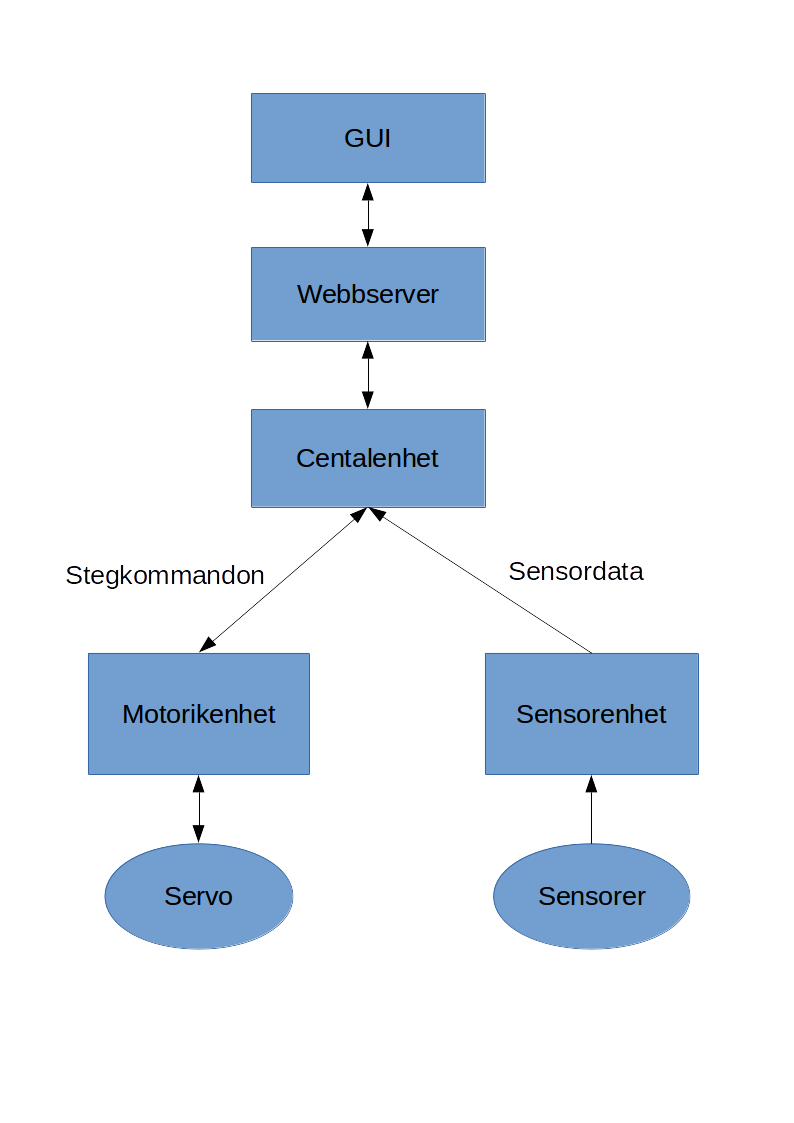
\includegraphics[width=0.5\linewidth]{images/overview.png}
		\caption{Översikt av systemet\label{fig:overview}}
	\end{figure}

	\subsection{Grov beskrivning av systemet}
	Här var det text här var det text här var det text
	här var det text här var det text här var det text
	här var det text här var det text här var det text.
	
	
	\subsection{Ingående delsystem}
	Här var det text här var det text här var det text
	här var det text här var det text här var det text
	här var det text här var det text här var det text.
	
	
	\section{Centralenheten}
	Här var det text här var det text här var det text
	här var det text här var det text här var det text
	här var det text här var det text här var det text.
	
	
	\section{Motorikenheten}
	Här var det text här var det text här var det text
	här var det text här var det text här var det text
	här var det text här var det text här var det text.
	
	
	\section{Sensorenheten}
	Här var det text här var det text här var det text
	här var det text här var det text här var det text
	här var det text här var det text här var det text.

\end{document}